\documentclass[noauthor,nooutcomes,hints,handout]{ximera}

%% page layout
\usepackage[in,headings]{fullpage}
\raggedright
\setlength\headheight{13.6pt}


%% fonts
\usepackage{euler}

\usepackage{FiraMono}
\renewcommand\familydefault{\ttdefault} 
\usepackage{mathastext}
\usepackage[htt]{hyphenat}

\usepackage[T1]{fontenc}
\usepackage[scaled=1]{FiraSans}

\usepackage{wedn}
\usepackage[T1]{fontenc}

%% wrap text around scripts
\usepackage{wrapfig}

\tikzset{>=stealth}
%% snap! scripts
\usepackage{scratch3}

\usepackage{adjustbox}

%% journal style
\makeatletter
\newcommand\journalstyle{%
  \def\activitystyle{activity-chapter}
  \def\maketitle{%
    \addtocounter{titlenumber}{1}%
                {\flushleft\small\sffamily\bfseries\@pretitle\par\vspace{-1.5em}}%
                {\flushleft\LARGE\sffamily\bfseries\thetitlenumber\hspace{1em}\@title \par }%
                {\vskip .6em\noindent\textit\theabstract\setcounter{question}{0}\setcounter{sectiontitlenumber}{0}}%
                    \par\vspace{2em}
                    \phantomsection\addcontentsline{toc}{section}{\thetitlenumber\hspace{1em}\textbf{\@title}}%
                     }}
\makeatother



%% thm like environments
\let\question\relax
\let\endquestion\relax

\newtheoremstyle{QuestionStyle}{\topsep}{\topsep}%%% space between body and thm
		{}                      %%% Thm body font
		{}                              %%% Indent amount (empty = no indent)
		{\bfseries}            %%% Thm head font
		{)}                              %%% Punctuation after thm head
		{ }                           %%% Space after thm head
		{\thmnumber{#2}\thmnote{ \bfseries(#3)}}%%% Thm head spec
\theoremstyle{QuestionStyle}
\newtheorem{question}{}



\let\freeResponse\relax
\let\endfreeResponse\relax

%% \newtheoremstyle{ResponseStyle}{\topsep}{\topsep}%%% space between body and thm
%% 		{\wedn\bfseries}                      %%% Thm body font
%% 		{}                              %%% Indent amount (empty = no indent)
%% 		{\wedn\bfseries}            %%% Thm head font
%% 		{}                              %%% Punctuation after thm head
%% 		{3ex}                           %%% Space after thm head
%% 		{\underline{\underline{\thmname{#1}}}}%%% Thm head spec
%% \theoremstyle{ResponseStyle}

\usepackage[tikz]{mdframed}
\mdfdefinestyle{ResponseStyle}{leftmargin=1cm,linecolor=black,roundcorner=5pt,frametitlefont=\wedn\bfseries,%frametitle={\underline{\underline{Response}}:}
, font=\wedn\bfseries,}%\begin{mdframed}[style=mystyle]foo\end{mdframed}


\ifhandout
\NewEnviron{freeResponse}{}
\else
%\newtheorem{freeResponse}{Response:}
\newenvironment{freeResponse}{\begin{mdframed}[style=ResponseStyle]}{\end{mdframed}}
\fi



%% attempting to automate outcomes.

\newwrite\outcomefile
  \immediate\openout\outcomefile=\jobname.oc
\renewcommand{\outcome}[1]{\edef\theoutcomes{\theoutcomes #1~}%
\immediate\write\outcomefile{\unexpanded{\outcome}{#1}}}

%% \newcommand{\outcomelist}{\begin{itemize}\theoutcomes\end{itemize}}



%% my commands

\newcommand{\snap}{{\bfseries\itshape\textsf{Snap!}}}
\newcommand{\flavor}{\link[\snap]{https://snap.berkeley.edu/}}


\usepackage{tkz-euclide}
\tikzstyle geometryDiagrams=[rounded corners=.5pt,ultra thick,color=black]
\colorlet{penColor}{black} % Color of a curve in a plot


\title{Platonic solids}
\author{Bart Snapp and Jenny Sheldon}

\begin{document}
\begin{abstract}
  We study solids, and learn facts whose origins are both old and new.
\end{abstract}
\maketitle

\begin{listOutcomes}
\item Explain what a Platonic solid is.
\item Identify Platonic solids.
\item Explain why there are only five Platonic solids.
\item Discover basic facts about Platonic solids.
\item Use basic vocabulary involving polyhedra.
\end{listOutcomes}


Around $2400$ years ago, there was a group of mystics---today we might
call it a cult---who called themselves the
\textit{Pythagoreans}.\index{Pythagoreans@The Pythagoreans} Being
mystics, the Pythagoreans had some strange ideas, but on the other
hand they were an enlightened group of people because they believed
that they could better understand the universe around them by studying
mathematics. As part of the Pythagoreans' numerological religion, they
thought that some polyhedra had special powers. The Pythagoreans
associated the following polyhedra to elements of nature:
\begin{center}\index{convex polyhedra!regular}\index{polyhedra!convex regular}
\begin{tabular}{|c|c|}
\hline
Fire: Tetrahedron & Air: Octahedron \\
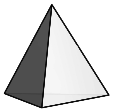
\includegraphics{tetrahedron.pdf} 
& 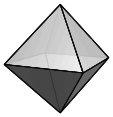
\includegraphics{octahedron.pdf} 
\\
\hline 
 Earth: Cube & Water: Icosahedron \\
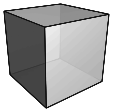
\includegraphics{cube.pdf} 
& 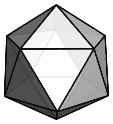
\includegraphics{icosahedron.pdf}  
\\
\hline
\end{tabular}
\end{center}
While the idea that these polyhedra are somehow connected to ``arcane
elements of nature'' is complete nonsense, there is actually something
special about the solids above. They are \textit{regular convex
  polyhedra}. Let's dissect those last words:

\begin{definition}\index{polyhedron} 
A \textbf{polyhedron} is a three dimensional solid that is bounded by
a finite number of polygons.
\end{definition}

\begin{definition}\index{convex} 
An object is \textbf{convex} if given any two points inside the object,
the segment connecting those two points is also contained inside the
object.
\end{definition}

\begin{definition}\index{regular!polyhedron} 
A polyhedron is \textbf{regular} if all its faces are the same regular
polygon and if the same number of polygons meet at every vertex.
\end{definition}

Apparently the Pythagoreans discovered the above four regular convex
polyhedra first. Only later did they discover a fifth, the
dodecahedron:
\begin{center}
\begin{tabular}{|c|}
\hline
\AE ther: Dodecahedron\\
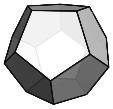
\includegraphics{dodecahedron.pdf} 
\\
\hline
\end{tabular}
\end{center}
Since the first four regular convex solids had elements associated to
them, the Pythagoreans reasoned that this fifth solid must also be
associated to an element. However, all the elements were accounted
for. So the Pythagoreans associated the dodecahedron to what we might
call the \index{aether@\ae ther}\ae ther, a mysterious non-earthly
substance.





\mynewpage






\begin{question}
  Consider the \index{triangular dipyramid}\textbf{triangular
    dipyramid}, the solid where two tetrahedrons are joined at a face:
  \[
  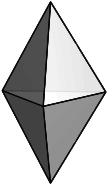
\includegraphics{triangulardipyramid.pdf}
  \]
  Is this a regular convex polyhedron? Explain your reasoning.
\end{question}

\mynewpage

\begin{question}
  There are at most five regular convex polyhedra. Let's (meaning you)
  explain why! I'll talk you through it.
  \begin{enumerate}
    \item Imagine a ``corner'' of a three-dimensional object made of
      polygons. What's the \textbf{minimum} number of faces required to make a corner? Is there a \textbf{maximum}?
    \item Start with a equilateral triangle. How many different
      ``corners'' can you make with it? (A $3$-faced corner? A
      $4$-faced corner? Keep going!)
    \item Now move on the square.  How many different ``corners'' can
      you make with it?
    \item Now move on the pentagon.  How many different ``corners'' can
      you make with it?
    \item Now move on the hexagon.  How many different ``corners'' can
      you make with it?
    \item What about other regular $n$-gons, how many different
      ``corners'' can you make with them?
    \item Explain why can be at most five regular convex polyhedra.
  \end{enumerate}
  
\end{question}

\mynewpage

\begin{question}
  The five regular convex polyhedra came to be known as the
  \index{Platonic Solids}\textbf{Platonic Solids} over 2000 years ago
  when Plato discussed them in his work \textit{Timaeus}. Here is an
  empty table of facts about the Platonic Solids---could you be so kind
  and fill it in?\index{Platonic Solids}
  \begin{center}
    {
      \renewcommand{\arraystretch}{3}
      \begin{tabular}{|l||c|c|c|c|}\hline
        Solid & Vertices & Edges & Faces & $V - E + F$\\
        \hline\hline
        Tetrahedron &  &   &  &   \\ \hline
        Octahedron &   &  &  &  \\ \hline
        Cube &  &   &  & \\ \hline
        Icosahedron &  &  &  & \\ \hline
        Dodecahedron &  &  &  & \\ \hline
\end{tabular}}
\end{center}
\end{question}



\end{document}
